%Classe du document, A4, police taille 12
\documentclass[a4paper,12pt]{article}

% Dictionnaire français, pour caractères spéciaux, tirets, caractères accentués
\usepackage[french]{babel}
\usepackage[linesnumbered,ruled,vlined]{algorithm2e}
\usepackage[utf8]{inputenc}
%Toujours plus d'accents
\usepackage[T1]{fontenc}

\usepackage{indentfirst}
%Pour créer des paragraphes random
\usepackage{lipsum}
%bibliographie
%Le style dépend du projet, voir avec le grand chef
%A mettre à l'endroit où vous voulez la faire apparaitre
%Donc dans le code pas ici t'as vu
%\bibliographystyle{ieeetr}
%\bibligraphy{nom_du_fichier.bib}

%hauteur entre deux lignes
\baselineskip 200cm
%hauteur entre deux paragraphes
\parskip 2mm
%longueur d'indentation
\parindent 2mm
%(on utilise \indent et \noindent sinon)

%Gérer ses marges

%Facilement
\usepackage[margin=2cm]{geometry}

%Précisément
%\usepackage[left=2cm , right=2cm, bottom=2cm, top=2cm, headheight=2cm]{geometry} 
%header c'est l'en-tête pas la marge supérieure

%Toujours plus précisément
%\addtolength{\oddsidemargin}{-0.5in}
%\addtolength{\evensidemargin}{-5cm}
%\addtolength{\topmargin}{-0.5in}

%Faires des articles  plusieures colonnes
\usepackage{multicol}
%Separation des colonnes
\setlength{\columnsep}{2cm}

%Avoir des entêtes et pieds de page stylés
\usepackage{fancyhdr}
\pagestyle{fancy}
%Pour enlever l'entête avec les sections
%\fancyhf{}

%Ca se fait sous format \<pos><type>{<contenu>}
%type c'est "head" ou "foot"
%pos pour position gauche "l", droite "r" ou centre "c"
%contenu c'est ce que tu mets dans dedans 
%marche aussi avec des images mais flemme
%mettre un trait
%\renewcommand{\footrulewidth}{1.5pt}

% Liens dans le document
\usepackage{hyperref}  
% Légendes dans les environnements "figure" et "float"
\usepackage{subcaption}
%La base pour faire des figures juste
\usepackage{graphicx}
\usepackage[export]{adjustbox}
\usepackage{wrapfig}
%Trucs utiles pour les maths
\usepackage{amsmath}

\begin{document}
\begin{titlepage}
    \begin{center}
        \vspace*{0.5cm}
        
\includegraphics[scale=0.1]{logo_ponts}\\
        \vspace{0.7cm}
        {\Large ÉCOLE NATIONALE DES PONTS ET CHAUSSÉES}\\
        \vspace{1cm}
        \rule\linewidth{0.05cm}
        {\huge Rapport de projet : KAHMATE \par}
        \rule\linewidth{0.05cm}
        \vspace{1cm}
        {\Large Technique de développement logiciel \par}
        \vspace{0.8cm}
        {\Large Par}\\
        \vspace{0.3cm}
        {\large \textit{ESTEVE Erwann}}\\
        \vspace{0.3cm}
        {\large \textit{FOURREAU Félix}}\\
        \vspace{0.3cm}
        {\large \textit{GOURGUE François}}\\
        \vspace{0.3cm}
        {\large \textit{DE MONICAULT Vianney}}\\
        \vspace{1.2cm}
    \end{center}
\end{titlepage}

\section{Menu principal}

Avant le lancement du jeu (\texttt{main()}), l'utilisateur se retrouve sur un écran de sélection. Il consiste en une fonction \texttt{main\_menu()} sous forme d'une boucle pouvant être quittée seulement lorsque l'option "QUIT" est sélectionnée.
Les 3 boutons à l'écran ("PLAY", "RULES" et "QUIT") sont des éléments de la classe \texttt{Button} de \texttt{main\_menu\_Button.py}. Cette classe consiste en un texte qui peut être associé à une image, et contient trois méthodes :



\begin{itemize}
  \item \texttt{Button.update(self, screen)}, qui fait apparaitre le texte et l'image à l'écran.
  \item \texttt{Button.checkForInput(self, position)}, qui vérifie si la coordonnée "position" (généralement la position du curseur) est dans le rectangle de Button.
  \item \texttt{Button.changeColor(self, position)}, qui fait changer la couleur du texte (par exemple dans le cas où le curseur passe au dessus du Button).
\end{itemize} 
Si l'évènement \texttt{pygame.MOUSEBUTTONDOWN} est activé (click souris), les collisions avec les boutons sont vérifiées :
\begin{itemize}
  \item Dans le cas où le bouton "PLAY" est pressé, \texttt{main()} est executée et le jeu commence. Lorsque la partie est terminée, l'utilisateur est ramené au menu principal.
  \item Dans le cas où le bouton "RULES" est pressé, \texttt{option()} est executée. Il s'agit d'une nouvelle page où les règles sont expliquées, il est possible de naviger parmis 7 pages associées à 7 fonctions \texttt{option()}. Lorsque le bouton "BACK" est pressé, \texttt{main\_menu()} est executé et l'utilisateur retourne sur le menu principal.
  \item Dans le cas où "QUIT" est pressé, la fenêtre se ferme.
\end{itemize}

\begin{figure}[h!]
  \centering
  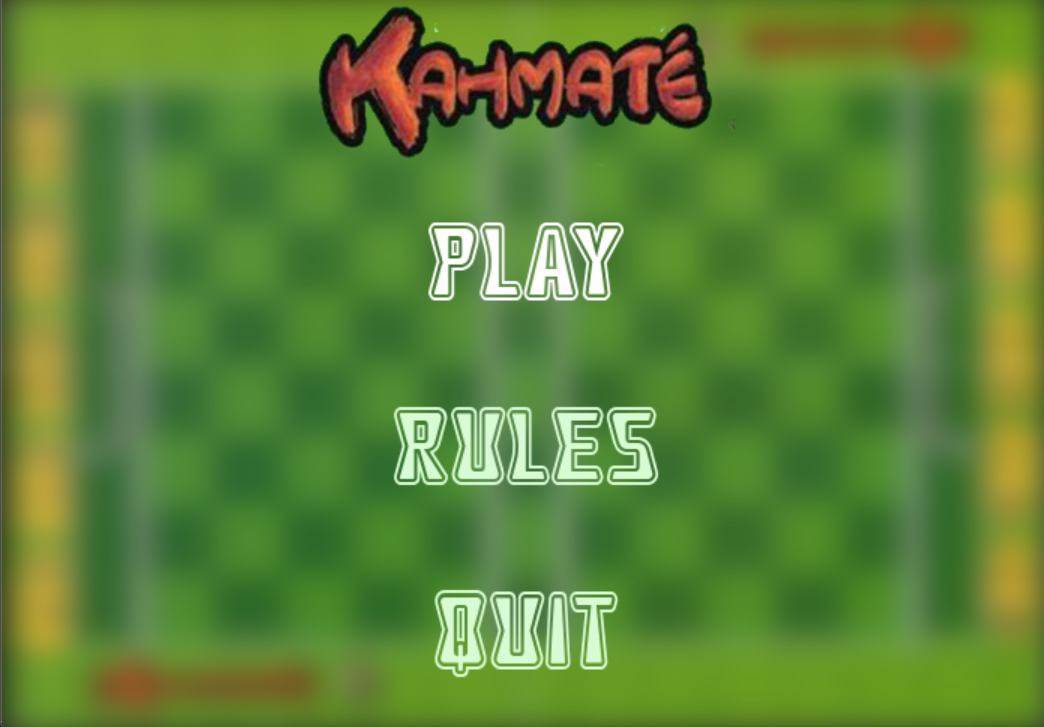
\includegraphics[width=0.45\linewidth]{main_menu_1.png}
  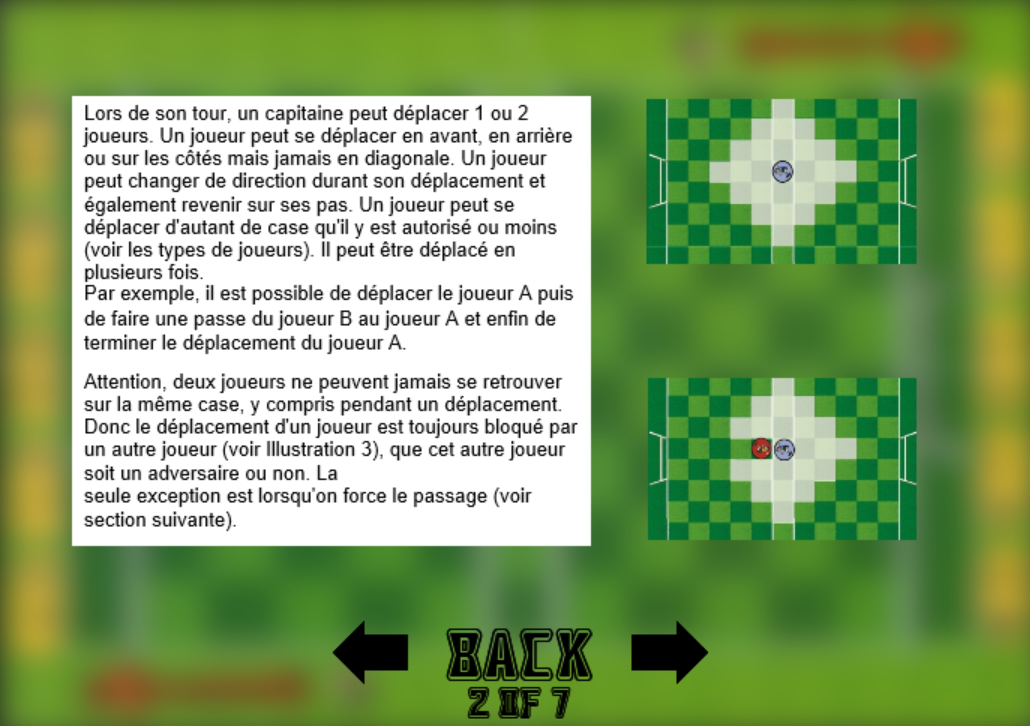
\includegraphics[width=0.45\linewidth]{main_menu_2.png}
  \caption{Le menu principal à gauche avec un des menu de règles}
\end{figure}

\section{Bot utilisant le Deep Reinforcement Learning}

L'idée de ce bot est de combiner les fonctionnalités du Deep Learning et du Reinforcement Learning.


D'une part, un réseau de neurones permet d'estimer la Q-valeur Q(s,a) d'une action a à partir d'un état s donné. La Q-valeur permet d'estimer la pertinence d'une action dans un état donné: plus elle est élevée, plus l'action est bonne et maximise les chances de gagner la partie.


D'autre part, le Reinforcement Learning permet de trouver fournir une estimation plus précise de la Q-valeur Q(s,a) d'une action à partir des estimations des Q-valeurs par le réseau de neurones. Cette estimation plus précise de la Q-valeur est ensuite retournée au réseau de neurones afin de mettre à jour ses paramètres afin d'améliorer ses prédictions.

L'équation de Reinforcement Learning utilisée est la suivante:\\

$Q(s_{t},a_{t}) = Q(s_{t},a_{t}) + \gamma \max_{a_{t+1} \in A_{t+1}} Q(s_{t+1},a_{t+1})$
\newline

où:
\begin{itemize}
    \item $s_{t}$ est l'état actuel de la partie
    \item $a_{t}$ est l'action choisie par le bot
    \item $s_{t+1}$ est l'état suivant après avoir effectué l'action $a_{t}$
    \item $A_{t+1}$ est l'ensemble des actions légales pour le bot dans l'état suivant
    \item $\gamma$ est le facteur de remise. Proche de 0 il prend peu en compte les états lointains, proche de 1 il y est sensible.
\end{itemize}
Il serait bien trop complexe de parcourir toutes les actions possibles dans chaque état et d'apprendre tout de suite tout ce qu'on peut apprendre sur chacune de ces actions. L'algorithme utilise préfère travailler avec des épisodes. Le bot joue donc avec sa stratégie toute une partie. Une fois la partie finie, chaque action choisie par le bot est analysée par l'algorithme de Reinforcement Learning puis sert d'entrainement pour le réseau de neurones.

Afin de traduire l'état de la partie et une action d'une manière compréhensible pour le réseau de neurones, on traduit un état de la partie par un tableau 2D ayant les dimensions de la grille de jeu. Les cases où se trouvent des rugbyman contiennent les nombres -1, -2, -3, -4, -5, 1, 2, 3, 4, 5 selon le type de rugbyman et le joueur (nombres négatifs pour le joueur rouge, nombres positifs pour le joueur bleu). On ajoute 0.5 dans la case où se trouve la balle. Les autres cases contiennent des 0.\\
Une action est également traduite comme un tableau 2D ayant aussi les dimensions de la grille de jeu. Si l'action est un déplacement de rugbyman, la case d'où part le rugbyman contient -1 et celle où il arrive contient 1. Si on déplace la balle, la case de départ contient -10 et la case d'arrivée contient 10. Toutes les autres cases contiennent des 0.\\

\section{Bot 'traditionnel'}
L'idée de ce bot est de déterminer quelle action choisir sans apprendre de ses parties passées.\\
Il faut donc pour cela quantifier chaque situation dans la partie et pouvoir calculer l'action optimale à effectuer en fonction de la situation décrite. POur cela on s'appuie sur une fonction de calcul de récompense rudimentaire. Celle-ci en fonction de qui a la balle va décrire des résultats différents. Si le bot a la balle, les récompenses vont croître vers la ligne d'essai et décroître a proximité des ennemis adverses; sinon, les récompenses vont croître vers la balle, qu'elle soit possédée par l'ennemi ou non. La stratégie du bot est alors relativement simple:
\begin{algorithm}[h!]
  \caption{Traditional Bot}
  \KwData{Game state}
  \KwResult{Bot's move}
  \textit{S} $\leftarrow$ Indicator of ball ownership\;
  \textit{R} $\leftarrow$ Reward map\;
  \If{S=1, the bot has the ball}{
    \textit{Rugbymen} $\leftarrow$ List of rugby players sorted by the best attainable reward\;
    \If{Owner = Rugbymen[0]}{
      Move the owner\;
      Move Rugbymen[1]\;
      End of turn\;
    }
    \Else{
      \For{Rugbyman in Rugbymen}{
        \If{Owner can pass to Rugbyman}{
          Owner passes to Rugbyman\;
          \textbf{break}\;
        }
      }
      Move the remaining rugby players according to the order of \textit{Rugbymen}\;
    }
  }
  End of turn\;
  \If{S=0, nobody has the ball}{
    \For{Rugbyman in Rugbymen}{
      \If{the ball is reachable by Rugbyman}{
        Move Rugbyman to the ball\;
        \If{Rugbyman can still move}{
          Move Rugbyman to the best reward\;
          \textbf{break}\;
        }
        \Else{
          \textbf{break}\;
        }
      }
    }
    \textit{Rugbymen} $\leftarrow$ List of rugby players sorted by the best reward\;
    Move the remaining rugby players according to the order of \textit{Rugbymen}\;
  }
  \If{S=-1, the enemy has the ball}{
    \textit{Rugbymen} $\leftarrow$ List of rugby players sorted by the best reward\;
    Action of \textit{Rugbyman}[0]\;
    \textit{S} $\leftarrow$ Indicator of ball ownership\;
    \If{S=1, we have recovered the ball}{
      Execute \textbf{3}\;
    }
    \Else{
      Action of \textit{Rugbymen}[1]\;
    }
  }
  \Return{Game instance}\;
\end{algorithm}
\newpage
\section{Element non présent dans la version finale}
\subsection{Menu flottant}
Initialement, les interractions entre l'utilisateur et les jetons de joueurs se faisaient via un menu flottant s'affichant à coté de la case contenant le jeton.
Ces menus étaient gérés par la classe \texttt{FloatingMenu} définie dans \texttt{menu.py}. 
La classe était fonctionnelle, mais nous avons préféré permettre au joueur de directement sélectionner les options via un click sur le jeton ou sur le ballon.



\end{document}
